\documentclass{article}
\usepackage{pgffor}
\usepackage{filecontents}
\usepackage{pdfpages }
\usepackage{graphicx} 
\usepackage{a4wide}
\usepackage{here} 
\usepackage{tabularx}
\usepackage[colorlinks]{hyperref}
\usepackage[german]{babel}
\usepackage[utf8]{inputenc}
\usepackage[T1]{fontenc}
\usepackage[3D]{movie15}
\usepackage{booktabs} 
\usepackage{eurosym}
\usepackage{verbatim}
\usepackage{amsmath}
\usepackage{textcomp}
\usepackage{caption}
\usepackage{setspace} 
\usepackage{geometry}
\geometry{a4paper, top=25mm}

\setcounter{tocdepth}{5}  % Ebenen für Aufnahme in das Inhaltsverzeichnis
\setcounter{secnumdepth}{4}  % Ebenen für Nummerierung


\begin{document}

\begin{titlepage}

\begin{center}
% Oberer Teil der Titelseite:
\includegraphics[width=0.15\textwidth]{../Files/logo.png}\\[1cm]    

\textsc{\LARGE Design-Dokument}\\[1.5cm]

\textsc{\Large Bremen}\\[0.5cm]


% Title
\newcommand{\HRule}{\rule{\linewidth}{0.5mm}}
\HRule \\[0.4cm]
{ \huge \bfseries Team Gamma}\\[0.4cm]

\HRule \\[1.5cm]

% Author and supervisor
\begin{minipage}{0.4\textwidth}
\begin{flushleft} \large
\emph{Autoren:}\\
Robin \textsc{Bley}\\
Alexander \textsc{Brennecke}\\
Alexander \textsc{Feldmann}\\
Marc \textsc{Huisinga}\\
Kevin \textsc{Neumeyer}\\
Till \textsc{Schlechtweg}\\
Steffen \textsc{Wißmann}
\end{flushleft}
\end{minipage}
\hfill
\begin{minipage}{0.4\textwidth}
\begin{flushright} \large
\emph{Betreuer:} \\
Harm \textsc{Hörnlein-Roboom}\\
Frank \textsc{Marschall}
\end{flushright}
\end{minipage}

\vfill

% Unterer Teil der Seite
{\large \today}

\end{center}

\end{titlepage}

\newpage
\thispagestyle{empty}
\tableofcontents
\thispagestyle{empty}
\newpage
\setcounter{page}{1}

% Import der Einleitung
\include{./1_Einleitung/einleitung_doku}

% Import der Hardware Doku
\section{Beschreibung des CanSat}


% Blockdiagramm (irgendjemand)
\subsection{Missionsüberblick}
Wir haben uns für den Satelliten überlegt, dass dieser so individuell wie möglich sein soll. Daher greifen wir nicht auf das vom Wettbewerb bereitgestellte T-Minus-CanSat-Kit zurück. Stattdessen haben wir uns im Detail überlegt, welche Sensoren unseren Erwartungen entsprechen und wie wir diese bestmöglich innerhalb der Dose platzieren können. Zusätzlich möchten wir nicht auf eine standardisierte Getränkedose als Hülle zurückgreifen, sondern auch hier unser eigenes Design erschaffen.

% 3D Skizze, Erklärung der einzelnen Bestandteile (Alexander B.)
\subsection{Mechanik- und Strukturdesign}

Wir haben den CanSat in drei Komponenten aufgeteilt: Die Hülle, die Innenwand und die Sensorikplatine. Diese drei Komponenten bilden den Hauptbestandteil des CanSats und haben maßgeblich zu dem mechanischen und strukturellem Design beigetragen. Im Nachfolgenden wird kurz auf jeden dieser Komponenten eingegangen und die exakte Funktion im Zusammenhang erklärt.

\subsubsection{Fachliche Grundlagen}
Um die 3D-gedruckte Wand zu erzeugen, wurde die 3D-Moddelierungssoftware \href{http://www.sketchup.com/de} {Sketchup} von Google verwendet. Sketchup bietet die Möglichkeit, vergleichsweise einfach 3D-Modelle zu zeichnen. Um dies zu tun, muss klar sein, welche Objekte gezeichnet werden sollen. Diese Objekte müssen vermessen und innerhalb von Sketchup gezeichnet werden. Dies erfordert die Kenntnis über gewisse mathematische Methoden zur Berechnung von Kreisen, Flächen und Körpern. Die meisten 3D-Drucker benötigen Dateien des Typs .stl, welche in Sketchup mit einem Plugin erzeugt werden können.
Zum Anfertigen von GFK-Komponenten wird ein Körper benötigt, auf welchen das GFK laminiert werden kann. In unserem Fall ist dieser Körper zylindrisch, mit einem Durchmesser von 31,5 mm, und aus Aluminium gefräst. \\
Um die Platine zu erstellen, wurde die Design-Software \href{http://www.cadsoft.de/eagle-pcb-design-software/} {Eagle PCB} verwendet. Eagle bietet die Möglichkeit, sowohl Schaltpläne als auch das entsprechende Layout zu erstellen. Im Anschluss wurde die Platine, mit Hilfe und Mitteln des \href{https://www.hackerspace-bremen.de/}{Hackerspace Bremen e.V.}, geätzt.

\subsubsection{Hülle}
Wir haben uns dazu entschieden, die äußere Hülle aus GFK (Glasfaser verstärkter Kunststoff) anzufertigen. Dieser hat die Eigenschaft, dass er bei einem sehr geringen Gewicht, und bei einer geringen Wandstärke, trotzdem eine gewisse Stabilität aufweist. Aus dem GFK haben wir eine Röhre mit einem Innendurchmesser von 31,5 mm und einem Außendurchmesser von 33,5 mm laminiert. Diese Röhre wurde auf eine Länge von 111 mm gekürzt und gefeilt. Um die Röhre oben und unten zu verschließen, haben wir uns bei \href{http://www.thyssenkrupp-system-engineering.com/de/home.html}{Thyssen Krupp System Engineering} zwei Aluminiumdeckel fräsen lassen. Diese haben uns ebenfalls durch ihr geringes Gewicht und ihre hohe Stabilität überzeugt. Die Deckel haben, genauso wie die Hülle, einen Außendurchmesser von 33,5 mm. Sie sind beide 2 mm dick und haben zusätzlich eine 2mm dicke Erhöhung, welche in die Röhre eingelassen wird. Eine Abbildung der Hülle kann unter \ref{pic_dose} gefunden werden.

\subsubsection{Innenwand}
Um die Elektronik innerhalb der Hülle zu platzieren und zu befestigen, haben wir uns dazu entschieden, eine Wand anzufertigen. Diese Wand teilt die Hülle mittig und bietet so auf beiden Seiten Platz, um unser Mikrokontrollerboard und unsere Sensorikplatine zu befestigen. Beide Bauteile werden mittels vier Gewindestangen an der Wand befestigt. Durch die Technik des 3D-Druckens ist es möglich, der Wand ein sehr geringes Gewicht bei einer verhältnismäßig hohen Stabilität zu verleihen. Zusätzlich gibt es uns die Möglichkeit, die Wand millimetergenau zu gestalten. Die Wand kann in ihrer finalen Form nur noch sehr schwer 3D gedruckt werden. Der Drucker muss dafür sogenannten ``Support'' drucken, welcher später wieder herausgeschnitten werden muss. Da dies die Druckzeit und die Qualität des Endproduktes vermindert haben wir uns dazu entschlossen die Wand vertikal zu zerteilen. Dadurch vermindert sich die Stabilität minimal, jedoch ist dieser Verlust so minimal, dass er zu vernachlässigen ist.\\

Am unteren Ende der Wand befindet sich eine Aushöhlung, sowie ein Fuß. Diese ist zum einen dafür da, um den Sharp-Feinstaubsensor zu befestigen. Zum anderen gibt der Fuß der Wand, und somit dem gesamten Satelliten, eine gewisse Stabilität. Der Fuß besitzt auf der einen Seite der Wand Bohrungen. Diese Bohrungen werden verwendet, um die Aluminiumdeckel an der Wand zu befestigen. An der oberen Seite der Wand befinden sich ebenfalls solche Bohrungen, um den oberen Deckel der Hülle zu befestigen. Da der Feinstaubsensor einen Luftzug benötigt, gibt es eine Bohrung, welche vertikal durch die Wand führt. Um das Mikrokontrollerboard mit der Sensorikplatine zu verbinden, existiert ein Fenster in der Mitte der Wand. Um die Sensorikplatine und das Mikrokontrollerboard an der Wand zu befestigen, existieren in der Wand weitere vier Bohrungen. Ein Bild der Wand kann unter \ref{pic_wand_3d} gefunden werden, während eine 3D-Darstellung der Wand unter \ref{pic_3d} gefunden werden kann.

\subsubsection{Sensorikplatine}
Die Sensorikplatine ist eine von uns geätzte Platine, welche mit unseren Sensoren bestückt ist. Es gibt mehrere positive Aspekte, die eine eigene Platine mit sich bringt. Zum einen bietet sie eine stabile Plattform für die Befestigung der Sensoren. Zum anderen sparen wir uns dadurch eine Menge Kabel, welche deutlich störanfälliger sind als eine Platine. Die Platine hat an den entsprechenden Stellen Bohrungen, um sie mit der Zwischenwand und dem Mikrokontrollerboard zu verbinden. Die Platine bietet Platz für die folgenden Module:

\begin{itemize}
	\item BMP108 Drucksensor: Misst den Luftdruck und gibt diesen, sowie die daraus berechnete Höhe, zurück
	\item Sparkfun UV Sensor: Misst die Intensität der Strahlung des Spektrums 270-380 nm, welches dem UVA und UVB Spektrum entspricht
	\item TMP006 Infrarot Temperatursensor: Misst die Temperatur eines dünnen Aluminiumstückes in der Außenwand 
	\item Adafruit Ultimate GPS: Bestimmt die aktuelle Position, sowie die Höhe
	\item APC220 Transceiver Modul: Sendet die Daten als JSON-String zur Bodenstation
	\item Steckplatz zum Anschluss des Sharp-Feinstaubsensors: Misst den Anteil der Partikel, welche kleiner als 10 \textmu m sind
	\item Steckplatz zum Anschluss an das Mikrokontrollerboard: Bildet die Schnittstelle zwischen BeagleBone und Sensorikplatine
\end{itemize}

Der Schaltplan der Sensorikplatine kann unter \ref{pic_schaltplan} gefunden werden, während das Layout der Platine unter \ref{pic_layout} gefunden werden kann.

\subsubsection{Batteriehalterung}
Als Stromversorgung wurden zwei Mignon-AA- Batterien gewählt. Diese liefern, pro Batterie 3,6V, und somit in Reihe geschaltet 7,2V. Die Batterien werden in eine standard Mignon-AA- Batteriehalterung platziert. Um diese Batteriehaltung in dem Design unterzubringen wurde eine dünne Platte per 3D-Druckverfahren angefertigt. Diese Platte kann über die beiden Female Pin-Layer des BeagleBone Black gelegt werden. Zur Befestigung dienen zwei Male Pin-Layer, welche durch Löcher in der 3D-Platte in das BeagleBone Black gesteckt werden können. Die Batteriehalterung wurde auf die 3D-Platte geklebt und zusätzlich mit Schrauben befestigt.

Diese Schrauben dienen ebenfalls dazu eine zweite Platine von unten an die 3D-Platte zu schrauben. Diese zusätzliche Platine ist mit einem Vorwiederstand, einer Z-Diode und einer Diode ausgestattet und dient dazu die Ausgangsspannung des BeagleBone Black zu reduzieren und zu glätten. Die 7,2V Ausgangsspannung können dadurch auf 5V reduziert werden, welche für das Transceiver Modul notwendig sind.

% Elektrisches Vorgehen, Schaltplan, Funkverbindung (Till)
\input {./2_Beschreibung_des_CANSAT/hardware_elektrischeKonstruktion_doku}

% Programmiersprache, Entwicklungsumgebung, abschätzung Datenmenge, Programmablauf (PAP), Datenverarbeitung (Steffen)
\subsection{Softwaredesign}
\subsubsection{Python als Programmiersprache}
Als Programmiersprache für das BeagleBone Black haben wir uns für Python entschieden. Es wäre ebenfalls möglich gewesen, den Mikrocontroller mit den Sprachen JavaScript, Java, C, C++, C\# und vielen weiteren Sprachen zu programmieren. Da es sich bei dem BeagleBone um ein Linux-basiertes Embedded System handelt, unterstützt es praktisch alle Programmiersprachen, sofern entsprechende Bibliotheken existieren. Allerdings haben wir uns aufgrund der Tatsache, dass Python im Gegensatz zu Java nicht objektorientiert geschrieben werden muss, für Python entschieden. Wir möchten auf der Hardwareseite möglichst auf objektorientierte Programmierung verzichten. Ein weiteres wichtiges Argument ist die gute Python-Bibliothek, welche von einer großen Community permanent gewartet und aktualisiert wird.
\subsubsection{Datenverarbeitung auf dem BeagleBone}
Die Datenverarbeitung auf dem BeagleBone verläuft relativ simpel. Zunächst werden alle von den Sensoren aufgezeichneten Daten, bei Sensoren mit I2C-Anbindung, mithilfe von Libraries, und bei den anderen mithilfe von Umrechnungsalgorithmen, gesammelt. Anschließend werden alle gesammelten Daten in einen JSON-String geparsed, welcher mithilfe von unserem Transceiver an die Bodenstation übermittelt wird. Diese übernimmt hieraufhin die weitere Verarbeitung und Darstellung der Messdaten. Zusätzlich werden die Daten auf dem internen Speicher des BeagleBones gespeichert. \\
Eine simple Skizze der Architektur lässt sich auch unter \ref{blockdiagramm} finden.

% Fallschirm (Alexander F.)
\subsection{Bergungssystem}
Für unser Landesystem haben wir uns entschieden, unseren eigenen Fallschirm zu bauen. Die Hauptaufgabe ist es, eine weiche Landung auf dem Boden zu garantieren. Unsere Vorgabe war, dass der Fallschirm und die Dose eine Fallgeschwindigkeit von 15 Meter/Sekunde haben soll. Leider sind unsere Testfallschirme, die wir auch schon im Vorjahr genutzt haben, für eine deutlich geringer Fallgeschwindigkeit ausgelegt. Dies haben wir uns zum Anlass genommen eine neue Fallschirmart zu testen. Die Idee dabei ist, dass die acht Schnüre, welche den Fallschirm an der Dose befestigen, mit sehr luftdurchlässigem Stoff, sogenannter Gaze, ersetzt werden. Wir erhoffen uns dadurch eine stabilere Lage in der Luft und ein fortschrittlicheres Design.

\subsubsection{Berechnungen}
Für den Bau des Fallschirm wissen wir bereits, dass dieser mit \(v = 15\frac{m}{s}\) fallen soll. Außerdem haben wir einen bereits berechneten Strömungswiderstandskoeffizient (\(C_w\)) von 1,33. Für die Berechnung des Fallschirms wurde folgende Formel verwendet:
\[
F_w = C_w \cdot \frac{1}{2} \cdot \rho \cdot v^2 \cdot A
\]
Fw ist die Strömungswiderstandskraft. Diese kann ermittelt werden, indem man die Fallwiederstandskarft einsetzt.
\[
F_w = m \cdot g = 350g \cdot 9,81\frac{m}{s^2} = 3,3433\frac{m}{s^2}kg
\]
Um die Größe des Fallschirms zu berechnen, kann man nun durch Einsetzen in die erste Formel diese nach A umstellen.
\[
A=\frac{2 \cdot 3,3433\frac{m}{s^2}kg}{C_w \cdot \rho \cdot v^2}
\]
\[
A=\frac{2 \cdot 3,3433\frac{m}{s^2}kg}{1,33 \cdot 1,2\frac{kg}{m^3} \cdot 15^2\frac{m^2}{s^2}} = 0,01862m^2 \text{ oder } 186,2cm^2
\]
Eine Fläche von 186,2 cm² entspricht einem Durchmesser von ca. 16 cm.

\subsubsection{Bau}
Beim Bau der Fallschirme haben wir den Stoff von Regenschirmen verwendet. Dieser Stoff ist sehr geeignet, da er bereits in einer Art Halbkugelform mit acht aneinandergefügten Panels ist. Er bietet genug Widerstand, um den Belastungen des Fluges standzuhalten und hat als praktischen Nebeneffekt, dass es regendicht ist. Um an den Stoff zu kommen muss das Gestell des Regenschirmes vorsichtig vom Stoff heruntergeschnitten werden. Danach muss in der Mitte des Stoffes, wo alle acht Kanten aufeinandertreffen, ein rund 5 cm großes Loch geschnitten werden. Dort kann die gestauchte Luft leichter entweichen, statt am Rand unkontrolliert auszutreten. Würde sie dies nicht tun, so könnte es leicht zu gefährlichen Turbulenzen kommen. Nun kann der Fallschirm in die entsprechende Größe zugeschnitten werden. Am Rand des Fallschirms sollte ein zusätzlicher ca. 1 cm breiter Rand gelassen werden, der in den Fallschirm umgeklappt wird. Dieser muss mit einer Nähmaschine auf den Fallschirm festgenäht werden. Dies dient dazu, die Struktur des Randes besser zu schützen. Am Rand besteht die höchste Wahrscheinlichkeit, dass durch eine kleine Kerbe ein kompletter Riss entstehen könnte. Auf dieser Grundlage kann nun die Gaze, auf dem Rand, genäht werden. Dabei sollte beachtet werden, dass beim Übergang von Fallschirm und Dose am Befestigungspunkt eine hohe Belastung auftritt. An diesem Punkt hat die Gaze einen gewaltigen Nachteil gegenüber der Schnüre. Hier kann es durch eine einmalige starke Belastung zum Riss kommen, der sich im Laufe des Fluges weiter ausbreiten kann. Daher haben wir uns dort dazu entschieden, eine Verstärkung mit einem sehr rissfesten Material einzunähen, der die Spannung erst kompensiert und diese nach dem Entfalten des Fallschirms gut auf die Gaze verteilt. Eine einfache Skizze des Fallschirms kann unter \ref{pic_fallschrimskizze} gefunden werden.

\subsection{Antenne}
Wir haben uns für den Bau einer Helixantenne entschieden. Diese hat gegenüber der Yagi-Antenne eine größere Verlässlichkeit beim Empfangen von Daten, da ihr Ausrichtungswinkel im Bezug auf den CanSat keine Rolle spielt und so durch die ständige Rotation des CanSats keine Daten verloren gehen können. Der größte Nachteil bei einer Helixantenne ist, dass sie eine fast 1m² große Bodenplatte besitzt. Da unsere Helixantenne von einer Person gehalten wird, haben wir darauf Wert gelegt, diese so leicht wie nur möglich zu bauen. Um das Gewicht der Antenne zu reduzieren, haben wir eine zwei Millimeter dicke Bodenplatte verwendet, was im Gegensatz zu oft verwendeten drei Millimeter dicken Bodenplatten ziemlich gering ist. Diese erfüllt, auch wenn sie nur ein Drittel der Empfangseffektivität besitzt, die benötigte Belastungsgrenze. Zusätzlich haben wir in die Bodenplatte, in einem symmetrischen Muster, viele kleine Löcher hineingebohrt. Mit diesen zahlreichen Löchern haben wir nochmals das Gewicht der Bodenplatte um ein Drittel reduziert. Die Löcher stören dabei nicht die Empfangseffektivität, da sie nur etwa ein Zehntel der Größe haben, die sie haben müssten, damit es Probleme beim Empfang gäbe.

\subsection{Aufgetretene Probleme}
Während des Baus des CanSats sind selbstverständlich einige Probleme aufgetreten. Manche dieser Probleme waren relativ leicht zu lösen, andere erforderten eine detaillierte Recherche. Im Nachfolgenden werden einige dieser Probleme und unsere Lösungsansätze erläutert.

\begin{itemize}
	\item \textbf{Befestigung der Dosendeckel}: Es war vorerst geplant, durchgängige Gewindestangen zu verwenden, welche durch die Wand führen und so die Deckel und die Wand miteinander verbinden. Diese Stangen kollidierten jedoch mit den Löchern für die Befestigung des Mikrokontorollers und der Sensorikplatine. Nach verhältnismäßig langem Überlegen und Ausprobieren haben wir uns dazu entschlossen, die Gewindestangen nicht durchgängig zu gestalten. Stattdessen werden sie lediglich durch den Fuß und den Kopf der Wand gesteckt und dort verschraubt. Dies hat den Vorteil, dass wir das Gewicht deutlich verringern und wir innerhalb des CanSats wesentlich mehr Freiräume haben, um Objekte zu platzieren. Nachteilig ist jedoch, dass dadurch die Stabilität verringert wird.
	\item \textbf{Spektrum des UV-Sensors}: Unser UV -Sensor misst die Intensität der Strahlung, welche im Spektrum 280-390 nm liegt. Dies hat die Folge, dass der Output des Sensors deutlich über dem zu erwartenden Wert liegt und es relativ schwer fällt, einen Vergleich zwischen diversen Messungen aufzustellen. Dies liegt daran, dass man nicht verifizieren kann, welche Wellenlänge mit welchem Anteil an dem Gesamtoutput beteiligt sind.
	\item \textbf{Intensität des Sharp-Feinstaubsensors}: Zunächst war der Sharp-Sensor dazu gedacht, die Feinstaubkonzentration in unserer Athmosphäre zu messen. Jedoch mussten wir feststellen, dass der Sensor keineswegs Feinstäube, sondern groberen Staub, wie zum Beispiel Hausstaub, misst. Dies stellte deshalb ein Problem dar, da wir bis dato das komplette Dosendesign auf den Sharp-Sensor abstimmten. Ein neuer Sensor war zwar verfügbar, konnte jedoch aufgrund des Dosendesigns nicht integriert werden, da dieser zu groß ist. Da es durchaus möglich ist mit dem Sharp-Sensor halbwegs akzeptable Werte zu erlangen, wenn man Referenzmessungen durchführt, bleibt dieser zumindest vorerst im Gesamtsystem erhalten.
	\item \textbf{Geeigneter Ozon-Sensor}: Es hat sich als äußert schwierig erwiesen, einen Ozon-Sensor zu finden, welcher keine lange Vorlaufzeit benötigt, verhältnismäßig klein ist und nicht übermäßig viel kostet. Daher ist es aktuell nicht mehr geplant, einen Ozon Sensor innerhalb des CanSats unterzubringen.
	\item \textbf{BeagleBone Black}: Zu Beginn unserer Arbeit am BeagleBone hatten wir einige Probleme mit diesem. Beispielsweise ließ sich zunächst die Python-Library für das BeagleBone nicht verwenden. Einige Pins ließen sich nicht ansteuern, was zu Fehlern führte. Letztlich fanden wir heraus, dass die Linux Distribution Debian auf dem System installiert war. Dieses ist jedoch für das BeagleBone Black noch in der Testphase und kann Bugs hervorrufen. Gelöst wurde das Problem, indem der Speicher mit dem Defaultsystem Linux Angstrom geflasht wurde. Danach funktionierte das Ausführen von Pythoncode ohne jegliche Probleme. Schließlich bootete das Beagle gegen Ende des Projektes nicht mehr und nach sorgfältiger Recherche im Internet stellte sich heraus, dass es sich um einen bekannten Fehler handelt, welcher allerdings mehrere Ursachen haben kann. Letztlich ist uns nicht bekannt weshalb das Beagle nicht mehr funkioniert, jedoch liegt die einzige Abhilfe in einem neuen Mikrocontroller. Da unser Dosendesign jedoch für das Beagle konzipiert wurde, blieb uns nichts anderes übrig als ein neues Beagle zu besorgen.
	\item \textbf{UART und I2C-Bus}: Bei der Übertragung mithilfe von UART und dem I²C-Bus sind wir auf Probleme in Kombination mit dem BeagleBone gestoßen. Dieses hatte verschiedene Ports und Protokolle standardmäßig nicht aktiviert. Wir mussten im Linux-System Angstrom einige Startroutinen hinzufügen, sodass bei jedem Start auch alle Ports und Protokolle aktiviert werden. Am Ende kostete dies viel Zeit, da die Dokumentation des BeagleBone in diesem Punkt nicht detailgenau war und für verschiedene Versionen verschiedene Lösungen des Problems existieren.
\item \textbf{Berechnung der Fallschirmgröße}: Das Ergebnis der Größenberechnung des Fallschirms erschien uns nicht realistisch. Der genutzte Cw-Wert hat einen Formfaktor, der nicht unseren Fallschirmen entsprach. Daher wurde beschlossen, einige Tests durchzuführen, um die Werte genauer zu bestimmen (siehe Testkonzept).
\item \textbf{Haltbarkeit des Gazestoffes}: Beim Bau des Fallschirms ist uns aufgefallen, dass der Stoff, der die Dose mit dem Fallschirm befestigt, eventuell nicht stark genug ist. Durch die sehr löchrige Struktur kann es schnell zu kleinen Rissen kommen. Werden diese zu stark belastet können diese sich ausbreiten.
\item \textbf{Durchmesser des CanSats}: Wir sind zu Beginn des Projektes davon ausgegangen, dass der Durchmesser des CanSats dem einer standardisierten Getränkedose entspricht (67mm). Zu spät ist uns aufgefallen, dass dies ein Irrtum war, und der Durchmesser 66mm betragen muss. Dies stellt jedoch kein Problem dar, da wir die Dicke der Außenwand problemlos um 0,5mm verringern können.
\item \textbf{Energieversorgung des Transceivers}: Das Transceiver-Modul unseres CanSats, ist das einzige Bauteil, welches eine 5V Spannungsversorgung benötigt. Dies stellte uns vor einige Probleme, da der 5V Output des Beagles lediglich die Betriebsspannung des Beagles ausgab, welche in unserem Fall bedingt durch die gewählten Batterien bei rund 7,2V lag. Dementsprechend würde eine überhöhte Spannung am Modul anliegen, welche dieses beschädigen würde. Letztlich wurde das Problem gelöst, indem die Spannung des Output-Pins mithilfe eines Vorwiderstandes und einer Z-Diode auf rund 5V reduziert wurde. Diese Lösung schließt Spannungsschwankungen, bedingt durch schwankende Stromstärken oder durch schwankende Eingangsspannungen am Beagle, nicht aus. Dies stellt jedoch kein Problem dar, da das Transceiver-Modul mit einer Spannung zwischen 3,5V und 5,5V arbeiten kann. Wollte man diese Schwankungen vollständig eliminieren, würde man um einen Spannungsregler nicht herum kommen, wobei mit erheblicher Verlustleistung zu rechnen wäre, welche wir nicht verkraften können da die Batterien in Bezug auf ihre Ladungsmenge bereits relativ knapp kalkuliert sind. 
\item \textbf{Unterbringung der Batterie}: Die Unterbringung der Spannungsversorgung unseres CanSats stellte uns gegen Ende des Projektes vor große Probleme, da wir der Unterbringung bis dato in unserem Dosendesign kaum Aufmerksamkeit geschenkt hatten. Letztlich gab es sogar Probleme ein Batteriefach für zwei Mignon-AA-Batterien unterzubringen. Dennoch schafften wir es mithilfe einer 3D-gedruckten Konstruktion das Batteriefach am Beagle selbst zu befestigen.
\item \textbf{Unterbringung des Schalters}: Nachdem das Problem der Unterbringung der Spannungsversorgung gelöst war, fiel uns auf, dass wir noch einen Hauptschalter benötigen. Letztlich lösten wir das Problem, indem wir ein Batteriefach für zwei Mignon-AA-Batterien mit einem Schalter verwendeten.
\item \textbf{Eine passende Batterie}: Einer der größten Nachteile am BeagleBone Black ist der vergleichsweise enorme Energiebedarf. Das Board benötigt im laufenden Betrieb ca. 200mA und während des Bootvorganges sogar kurzzeitig das Doppelte. Es gibt zwar eine Vielzahl an Lithium-Polymer (LiPo) Akkumulatoren, jedoch konnten wir keinen LiPo Akku finden, welcher die benötigte Stromstärke, Kapazität und Spannung mitbringt und zusätzlich eine Größe (bzw. ein Format) besitzt, welches sich in unser Dosendesign eingliedert. Dieses Problem wurde schlussendlich durch zwei Mignon-AA- Batterien gelöst (näheres im Entsprechenden Kapitel). Dies ist mit Sicherheit keine optimale Lösung, für uns jedoch bei weitem die Beste.
\item \textbf{Anschluss von UART und ADC Sensoren an den I²C-Bus}: Unser Plan war gewesen, alle Sensoren an den I²C-Bus anzuschließen. Daraus hätte sich ein softwareseitiger Vorteil ergeben, der die Entwicklung und die Geschwindigkeit der auf dem Mikrocontroller ausgeführten Software deutlich verbessert hätte. Jedoch entschieden wir uns aus verschiedenen Gründen dagegen. Zunächst würde jeder Sensor seinen eigenen Analog zu Digital Converter benötigen, was bei uns zu erheblichen Platzproblemen geführt hätte. Desweiteren standen wir unter zeitlichem Druck und andere Probleme erforderten dringlicher einer Lösung als die Optimierung der Übertragungsprotokolle.
\end{itemize}

\subsection{Testkonzept}
Um sicherzustellen, dass der CanSat problemlos funktioniert, wurden diverse Tests durchgeführt. Dazu zählt natürlich das Prüfen auf Funktionstüchtigkeit der Sensoren. Hierfür wurde jeder Sensor separat an verschiedene Mikrocontroller (BeagleBone Black, Arduino Mega) angeschlossen. Dadurch konnte verifiziert werden, dass jeder Sensor unter jedem Board den gleichen Output liefert. Zusätzlich wurde überprüft, ob die Sensoren auf eine Veränderung der zu messenden Eigenschaft reagieren. Um zu erkennen, ob die gemessenen Werte den tatsächlichen Werten entsprechen, werden diese im Umweltlabor von \href{https://www.atlas-elektronik.com/atlas-elektronik/}{Atlas Elektronik} getestet und kalibriert. Dort soll ebenfalls überprüft werden, wie stabil der CanSat ist, um vorherzusagen, ob er beim Aufschlag beschädigt wird. Das Testkonzept für die Sensoren beruht im Wesentlichen auf Trial and Error.

Die Antenne wird im \href{http://www.hf.uni-bremen.de/start/}{Labor für Hochfrequenztechnik an der Universität Bremen} durchgetestet. Hierzu wird die genaue Frequenz bestimmt, auf der die Antenne empfängt, und eine Impedanzanpassung durchgeführt.

Um den Fallschirm zu prüfen wurde ein Experiment durchgeführt. Dazu wurde die Zugkraft des Fallschirms gemessen. Aus einem Auto, welches mit einer Geschwindigkeit von 50 km/h fuhr, haben wir einige Testfallschirme an einem Newtonmeter befestigt und dieses aus dem Auto gehalten. Die Berechnung der Kraft sieht folgendermaßen aus:
\[
F = m \cdot g
\]
\[
F = 300g \cdot 9,81\frac{m}{s^2} \cdot \frac{1kg}{1000g}
\]
\[
F = 2,943 \frac{m}{s^2} kg
\]
Aus der Geschwindigkeit und dem Widerstand des Newtonmeters konnte ermittelt werden, dass der Fallschirm keine 30 cm Durchmesser benötigt. Weitere Tests haben ergeben, dass 16 cm ein besserer Wert ist. Bei einem Fallschirm dieser Größe können auch schon relative kleine Veränderung der Größe die Fallgeschwindigkeit enorm beeinflussen. \\
Beim Test der Fallschirmgröße ist uns aufgefallen, dass die Gaze bei mehreren Versuchen kleine Risse bekommen hat. Das Material, das wir verwendet haben, ist nicht stark genug, um die Belastungen während des Fluges zu tragen. Aus diesem Grund haben wir uns dazu entschieden, die Gaze komplett wegzulassen. Stattdessen verwenden wir, wie im letzten Jahr, acht Schnüre, die an der Dosendecke befestigt werden.

Um die Datenübertragung und die restlichen Features des CanSats zu überprüfen, wird das System als Ganzes getestet. Der CanSat wird eingeschaltet, die Antenne auf den CanSat gerichtet, die Bodenstation an die Antenne angeschlossen, die Satellitenkonfiguration eingestellt, der Hotspot der Bodenstation gestartet und die Android-App mit dem Hotspot verbunden. Anhand der einzelnen Komponenten der Datenübertragung (CanSat, Desktopapplikation, Android-Applikation) lässt sich etwa erkennen, an welcher Stelle der Übertragung Fehler auftreten. Funktioniert die Übertragung über alle Komponenten mit allen Sensoren, so ist der Test erfolgreich.

% Import der Bodenstation Doku
\input{./3_Beschreibung_der_Bodenstation/bodenstation_doku}

% Import der Projektplanung
\section{Projektplanung}
\subsection{Zeitplan der CanSat-Vorbereitung}
Die Zeitplanung ist ausgerichtet für den Zeitpunkt der Abgabe unseres P5-Projekts, da wir uns erhofft haben, zu diesem Zeitpunkt mit dem Projekt fertig zu sein. Dieser Zeitplan wurde jedoch von Anfang an sehr kritisch gesehen. Daher ist es nicht verwunderlich, dass der Fortschritt des Projektes geringer ist, als er zum jetzigen Zeitpunkt eigentlich sein sollte. Dies ist jedoch nicht dramatisch, da bis zum Wettbewerb genügend Zeit ist, die restlichen Arbeitspakete abzuarbeiten. Das gesamte Management der Arbeitspakete und des Zeitaufwandes wurde mit der Projektmanagementsoftware \href {www.redmine.org} {Redmine} erledigt. Da diese auf unserem Server unter \href{http://redmine.gamma-team.de}{redmine.gamma-team.de} erreichbar ist, kann jedes Teammitglied zu jedem Zeitpunkt den Fortschritt der Arbeit verfolgen. Die Planung der beiden Halbgruppen ist größtenteils voneinander getrennt. Es gibt jedoch gemeinsame Meilensteine, welche von beiden Gruppen eingehalten werden sollen. Bevor die Arbeit der Halbgruppen begonnen hat, gab es eine allgemeine Projektfindungsphase. In dieser Phase wurde ein grober Zeitplan festgelegt und es wurden alle relevanten Systeme (Webserver, Projektmanagementsoftware, GitLab etc.) aufgesetzt und eingerichtet um später einen reibungslosen Ablauf der Arbeitsphase zu garantieren. Die Idee und die Spezialisierung der Idee für das gesamte Projekt entstand ebenfalls in dieser Zeit. Anschließen wurde eine separate Zeitplanung in den beiden Halbgruppen erstellt, welche im Nachfolgenden erläutert wird.

\subsubsection{Zeitplan der Hardware-Gruppe}
Innerhalb der Hardwaregruppe wurde versucht, die meisten Aufgaben zu parallelisieren. Jedes Teammitglied hat sein eigenes spezielles Aufgabengebiet. Zwischen den Teammitgliedern herrscht trotzdem ein stetiger Austausch. Grund für die Parallelisierung war, dass in unseren Augen die meisten Aufgaben  nur die Aufmerksamkeit einer Person benötigen. Es ist nur selten erforderlich, dass mehrere Teammitglieder an demselben Arbeitspaket arbeiten müssen. Der gesamte Arbeitsprozess wurde in diverse Abschnitte gegliedert. Diese Abschnitte lassen sich auch im GANTT-Diagramm im Anhang dieses Dokumentes wiederfinden. Die einzelnen Abschnitte sind in diverse Arbeitspakete unterteilt, Personen zugewiesen und mit einem Zeitraum versehen. Bei den Abschnitten handelt es sich um folgende:
\begin{itemize}
\item Planung: Erstellung von Arbeitspaketen sowie eine Verteilung dieser und eine Erstellung diverser Diagramme
\item Fallschirm: Gestaltung und Bau des Bergungssystems
\item Sensorik: Heraussuchen, Bestellen und Testen passender Sensoren für unser Projekt
\item Beagleboard: Festlegung der Programmiersprache, IDE und der Recherche zu den elektrotechnischen Eigenschaften des Boards
\item Dose: Design und Bau der Hülle und der Deckel der Dose
\item Dosenmanagement: Design und Bau des Inneren der Dose sowie die Integration der Sensoren in das Gesamtsystem
\end{itemize}

Das GANTT-Diagramm der Hardware-Gruppe kann auch unter \ref{gantt_hardware} gefunden werden.

\subsubsection{Zeitplan der Software-Gruppe}
In der Softwaregruppe haben wir uns, wie in der Hardwaregruppe, dafür entschieden, die Aufgaben untereinander zu verteilen. Dabei haben wir zuerst die Bodenstation und die Android-Applikation komplett voneinander getrennt. Die Bodenstation war von Beginn an fester Bestandteil unseres Projektes. Die Android-App kam erst später hinzu und musste daher separiert behandelt werden. Noch vor dem eigentlichen Start des Projektes wurde diskutiert, wie die Software aufgebaut sein soll und welche Technologien für die Bodenstation verwendet werden kann. Nachdem die ersten Entscheidungen getroffen waren, haben wir angefangen, das Projekt in verschiedene Meilensteine zu unterteilen. Daraus ist folgende Gliederung entstanden:
\begin{itemize}
    \item Erstellung einer detaillierten Ticketübersicht
    \item Basisversion, mit allen Tickets, welche zur Bereitstellung der ersten Features nötig sind
    \item Export, mit allen Tickets, welche zum Exportieren von Daten nötig sind
    \item Kartenvisualisierung, mit allen Tickets, welche für das Darstellen des Satellitenfluges nötig sind
    \item Wissenschaftliche Analyse, mit allen Tickets, welche zur wissenschaftlichen Analyse der gesammelten Daten nötig sind
    \item Finale Version, mit allen Tickets, welche zur Zusammenführung der Bodenstation nötig sind
    \item RC 1 v1.1, mit allen Tickets, welche für den letzten Schliff der Bodenstation nötig sind
\end{itemize}
Innerhalb dieser Meilensteine haben wir das Projekt daraufhin in einzelne Tickets unterteilt. Jedes dieser Tickets spiegelt eine einzelne Aufgabe zur Fertigstellung der Bodenstation wieder. Diese Aufteilung hat es uns ermöglicht, die Aufgaben innerhalb der Bodenstation relativ flexibel zu verteilen. Dies hat dazu beigetragen, dass selten jemand auf eine andere Aufgabe warten musste. Die Tickets, welche sich innerhalb der Meilensteine befinden, haben sich während der Durchführung des Projektes immer wieder verändert. Dies war abhängig von den Ansprüchen, welche sich in dem jeweiligen Moment ergeben haben. Das im Anhang unter \ref{gantt_software} vorhandene GANTT-Diagramm gibt also nicht nur unsere Planung zum Anfang des Projektes wieder, sondern auch die kontinuierliche Präzisionsplanung während der Durchführung des Projektes.

Die Idee der App entstand deutlich später als die des restlichen Projektes. Daher wurde bei der Planung in Wochenschritten gedacht. Durch diese Methode konnten alle zwei Wochen kontrolliert werden, ob eine Komponente fertiggestellt ist. Falls mehr Zeit benötigt wurde, so war es möglich, am Wochenende an der Android-App zu arbeiten. Zusammengefasst existieren insgesamt sieben Arbeitspakete:
\begin{itemize}
	\item Der Debugger, der die Livedaten simulieren soll
	\item Liniengraph GUI
	\item Liniengraph Logic
	\item Balkendiagramm GUI
	\item Balkendiagramm Logic
	\item Optionen
	\item Menü
\end{itemize}

Das GANTT für die Android-Applikation lässt sich unter \ref{gantt_android} finden.

\subsection{Einschätzung der Mittel}
\subsubsection{Budget}
% \begin{tabular}{p{1,5cm}p{1,5cm}p{3,5cm}p{6,5cm}rrrl}
\label{subsubsec:Budget}

Um das CanSat Projekt zu finanzieren, konnten wir aktuell noch keine Sponsoren finden. Jedoch konnten wir uns mit unserem Schulverein verständigen, welcher uns finanziell unterstützen wird. Da wir nicht auf das T-Minus-Kit zurückgreifen, sondern stattdessen ein anderes Mikrokontrollerboard verwenden, können wir ungefähr 150\euro  sparen. Der 200\euro  Watterot Gutschein, welcher vom Wettbewerb gestellt wird, ist in unserer Rechnung noch nicht inbegriffen. Dies liegt daran, dass noch nichts bei Watterot bestellt wurde, bzw. die Bestellung lange vor der Annahme am Wettbewerb getätigt wurde.
Im Nachfolgenden sind alle Ausgaben und Einnahmen aufgelistet.
\begin{table}[H]
  \centering
    \begin{tabular}{p{1,7cm}p{1,5cm}p{3,5cm}p{6,5cm}rrrl}
    \toprule
    \textbf{Ausgabe} & \textbf{Datum} & \textbf{Empfänger} & \textbf{Grund} \\
    \midrule
    -12,16 \euro  & 08.01.2015 & Watterott & BMP180 Breakout \\
    -28,99 \euro  & 09.01.2015 & eBay - rcskymodel & Ultimate GPS \\
    -14,32 \euro  & 10.01.2015 & Spark Fun Electronics & UV-Sensor \\
    -51,99 \euro  & 10.01.2015 & Amazon & BeagleBone Black \\
    -17,30 \euro  & 01.12.2014 & eBay - hdt-preiswert & 
GFK-Set 1kg Polyesterharz + 20g Härter + $2m^2$ Glasfasermatte \\
    -3,54 \euro  & 23.03.2015 & toom baumarkt & 6 x Schleifpapier \\
    -3,79 \euro  & 23.03.2015 & toom baumarkt & Filzrolle \\
    -4,49 \euro  & 23.03.2015 & toom baumarkt & Plüschwalzen \\
    -2,19 \euro  & 23.03.2015 & toom baumarkt & Mundschutz \\
    -1,99 \euro  & 23.03.2015 & toom baumarkt & Farbwanne \\
    -4,99 \euro  & 23.03.2015 & toom baumarkt & Einmalhandschuhe \\
    -133,04 \euro  & 02.06.2015 & Alexander Brennecke& Rückzahlung bisheriger Ausgaben\\
	-139,80 \euro  & 23.03.2015 & Amazon & 2x BeagleBone Black\\
    \bottomrule
    - 145,75 \euro & & & \\
    \bottomrule
    \end{tabular}%
    \caption{Ausgaben}
  \label{tab:budgetausgaben}%
\end{table}%

\begin{table}[htbp]
  \centering
    \begin{tabular}{p{1,7cm}p{1,5cm}p{3,5cm}p{6,5cm}rrrl}
    \toprule
    \multicolumn{1}{c}{\textbf{Einnahmen}} & \textbf{Datum} & \textbf{Absender} & \textbf{Grund} \\
    \midrule
              17,30 \euro  & 01.12.2014 & Alexander Brennecke & GFK-Kauf \\
           107,46 \euro  & 10.01.2015 & Alexander Brennecke & Sensorenkauf \\
              20,99 \euro  & 23.03.2015 & Alexander Brennecke & toom Einkauf \\
133,04 \euro  & 02.06.2015 & Schulferein der Europaschule SII Utbremen & Sponsoring \\
    \bottomrule
    145,75 \euro & & & \\
    \bottomrule
    \end{tabular}%
	\caption{Einnahmen}
  \label{tab:budgeteinnahmen}%
\end{table}%

\subsubsection{Externe Unterstützung}
Externe Unterstützung erhielten wir von vielen Lehrern unserer Schule, welche uns Fragen zur Elektrotechnik und Softwareprogrammierung beantworten konnten. Zusätzlich haben wir finanzielle Unterstützung durch den Schulverein unserer Schule erhalten (siehe~\ref{subsubsec:Budget}).
Unterstützung außerhalb unserer Schule erhielten wir durch folgende Personen/Organisationen:

\begin{itemize}
	\item Das \href{https://www.hackerspace-bremen.de/}{Hackerspace Bremen e.V.}, welches uns ihren 3D-Drucker zur Verfügung gestellt hat. Zusätzlich konnten wir dort unsere Platine ätzen.
	\begin{comment}
	\item \href{http://de.wikipedia.org/wiki/Martin_Schneider_(Nachrichtentechniker)} {Prof. Martin Schneider} von von dem Hochfrequenzlabor der Universität Bremen, welcher uns geholfen hat unsere Antenne an die Frequenz und die Wellenimpedanz anzupassen.
	\end{comment}
	\item Das Umweltlabor der \href{http://www.atlas-elektronik.com/atlas-elektronik/}{Atlas Elektronik GmbH} hat uns geholfen, den CanSat, hinsichtlich seiner Stabilität, zu testen und die Sensoren korrekt zu kalibrieren.
\end{itemize}

% Import der Oeffentlichkeitsarbeit
\include{./5_Oeffentlichkeitsarbeit/oeffentlichkeitsarbeit_doku}

% Import der Anforderungen
\include{./6_Anforderungen/anforderungen_doku}

% Import der Reflexion
\include{./7_Reflexion_des_Projektverlaufes/projektverlauf_doku}

% Import des Anhanges
\section{Anhang}

\subsection{Einleitung}
\subsubsection{Blockdiagramm}
\begin{figure}[htbp]
	\centering
	\includegraphics[width=0.8\textwidth]{8_Anhang/Blockdiagramm.png}
	\caption{Blockdiagramm vom CanSat}
	\label{blockdiagramm}
\end{figure}

\newpage

\subsection{GANTT-Diagramme}
\subsubsection {Hardware-GANTT}
\begin{figure}[htbp]
	\centering
	\includegraphics[trim = 2mm 2mm 2mm 2mm, clip,width=0.8\textwidth]{8_Anhang/hardware-gantt-1.png}
	\label{gantt_hardware_1}
\end{figure}
\vspace{-2cm}

\newpage
\subsubsection {Bodenstation-GANTT}
\begin{figure}[H]
	\centering
	\includegraphics[trim = 25mm 50mm 46mm 65mm, clip,width=0.8\textwidth]{8_Anhang/bodenstation-gantt-1.png}
	\label{gantt_hardware_1}
\end{figure}
\vspace{-1,3cm}
\begin{figure}[H]
	\centering
	\includegraphics[trim = 30mm 50mm 45mm 40mm, clip,width=0.8\textwidth]{8_Anhang/bodenstation-gantt-2.png}
	\label{gantt_hardware_2}
\end{figure}
\vspace{-1,1cm}
\begin{figure}[H]
	\centering
	\includegraphics[trim = 30mm 200mm 45mm 40mm, clip,width=0.8\textwidth]{8_Anhang/bodenstation-gantt-3.png}
	\caption{Das GANTT-Diagramm der Bodenstation}
	\label{gantt_hardware_3}
\end{figure}
\newpage
\subsubsection {Android-App-GANTT}
\begin{figure}[H]
	\centering
	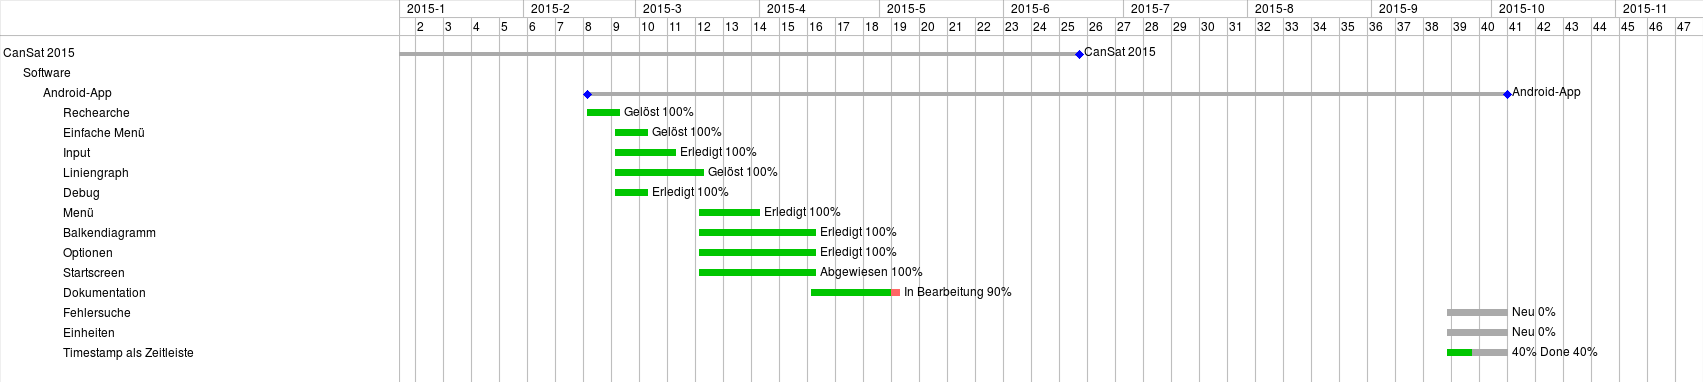
\includegraphics[trim = 30mm 200mm 45mm 40mm, clip,width=0.8\textwidth]{8_Anhang/android-app-gantt.png}
	\caption{Das GANTT-Diagramm der Android-App}
	\label{gantt_hardware_3}
\end{figure}

\newpage
\vspace{-2cm}
\subsection{Der CanSat}

\begin{figure}[H]
	\centering
	\includegraphics[trim = 11mm 335mm 20mm 210mm, clip, width=0.8\textwidth]{8_Anhang/dose.jpg}
	\caption{Die Hülle und ein Dosendeckel}
	\label{pic_dose}
\end{figure}

\begin{figure}[H]
	\centering
	\includegraphics[ width=0.8\textwidth]{8_Anhang/Wand_3D.PNG}
	\caption{Screenshot der Zwischenwand aus Sketchup}
	\label{pic_wand_3d}
\end{figure}

\newpage

\begin{figure}[h] 
      \centering 
      \includemovie[ 
        poster,controls,
       3Djscript=2_Beschreibung_des_CANSAT/Encompass.js
      ]{0.8\textwidth}{15cm}{2_Beschreibung_des_CANSAT/CanSat_2015.u3d} 
      \caption{Der Satellit (Diese Zeichnung ist möglicherweiße nicht sichtbar, da es eine 3D-Zeichnung ist. Bitte verwenden Sie den \href{https://get.adobe.com/reader/?loc=de}{Adobe Acrobat Reader})}\label{pic_3d} 
\end{figure} 

\newpage

\begin{figure}[H]
	\centering
	\includegraphics[trim = 60mm 100mm 55mm 100mm, clip, width=0.8\textwidth]{8_Anhang/Schaltplanv1.png}
	\caption{Der Schaltplan der Sensorikplatine}
	\label{pic_schaltplan}
\end{figure}

\newpage

\begin{figure}[H]
	\centering
	\includegraphics[trim = 200mm 300mm 200mm 280mm, clip,width=0.8\textwidth]{8_Anhang/Layoutv1.png}
	\caption{Das Layout der Sensorikplatine}
	\label{pic_layout}
\end{figure}

\newpage

\begin{figure}[H]
	\centering
	\includegraphics[ width=0.8\textwidth]{8_Anhang/fallschirmSkizze.PNG}
	\caption{Skizze des Fallschirms}
	\label{pic_fallschrimskizze}
\end{figure}

\newpage

\subsection{Bodenstationsnutzeranleitung}
\label{bodenstationsanleitung}
\subsubsection{Datenempfang}
Um Daten in Echtzeit zu empfangen, muss eine Verbindung zu einem Satelliten aufgebaut werden. Hierzu muss generell zu allererst ein Satellit erstellt werden. Hierfür wählt man unter dem Menüpunkt ``File'' den Unterpunkt ``Satellites'' aus. Dort ist es möglich, unter ``Add'', einen Satelliten hinzuzufügen. Um einen Satelliten zu laden, wählt man im selben Unterpunkt ``Manage'' aus. Dort wählt man den Satelliten aus, von welchem man Daten empfangen will. Anschließend sieht man einen Dialog mit Konfigurationsmöglichkeiten für den Datenempfang vom Satelliten (z. B. Serieller Port). Wenn man die Konfiguration abgeschlossen hat, beendet man den Dialog mit einem Klick auf ``Load configuration''. 
Möchte man den Datenempfangen beginnen, dann klickt man auf den ``Play''-Button in der Toolbar, welcher die Datenübertragung startet. Ab hier können verschiedene Visualisierungen geöffnet werden, um die empfangenen Daten darzustellen.
\subsubsection{Datenimport}
Um Daten aus einer Datei zu importieren, wird im Menüpunkt ``File'' der Untermenüpunkt ``Import'' ausgewählt. Anschließend wird eine Datei ausgewählt, welche importiert werden soll. Mit der Bestätigung werden die Daten dieser Datei eingelesen.
\subsubsection{Datenexport}
Für das Exportieren der Daten gilt, dass alle aktuell geladenen Daten exportiert werden. Darunter fallen entweder zwischengespeicherte Daten einer Liveübertragung, oder Daten, welche aus einer Datei importiert wurden.
Zum Exportieren der Daten wird im Menüpunkt ``File'' der Untermenüpunkt ``Export'' ausgewählt. Unter diesem Menüpunkt ist das Datenformat wählbar, in welches die gesammelten Daten gespeichert werden (Beim Graphenexport ist es wichtig, dass die Graphenvisualisierung während des Vorgangs geöffnet ist). Anschließend ist ein Pfad und ein Name wählbar, unter dem die Datei gespeichert wird. Mit der Bestätigung werden die Daten exportiert.
\subsubsection{Datenweiterleitung}
Per Klick auf das rote runde Icon in der Toolbar wird ein Hotspot-Server gestartet. Dieser sendet empfangene Daten in Echtzeit an alle Clients weiter, die mit dem Hotspot-Server verbunden sind.
\subsubsection{Oberflächenpersonalisierung}
Der Oberfläche können einzelne Komponenten hinzugefügt und entfernt werden. Diese Komponenten können unterschiedlich angeordnet werden. Um Visualisierungs-Komponenten hinzuzufügen wird unter dem Menü ``Window'' eine Visualisierung ausgewählt.
Um einen der bestehenden Komponenten zu entfernen wird das Kreuz angeklickt, welches sich am Tab des Komponenten befindet. Per ``drag and drop''  können diese Komponenten neu angeordnet werden, dazu muss der Tab des Komponenten ausgewählt werden. In verschiedenen Bereichen können Komponenten angeheftet oder verschoben werden. Außerdem können diese übereinander verlagert werden um sie in verschiedenen Tabs und in dem selben Bereich zu verwalten.

\subsubsection{Kartenvisualisierung}
Die Kartenvisualisierung startet über den Untermenüpunkt ``Map Visualization'' im Menüpunkt ``Window''. Geladene Werte werden dort angezeigt. Einzelne Messpunkte sind mit einem Punkt gekennzeichnet und mit einer Linie verbunden, was den Flugweg des Satelliten anzeigt.

\subsubsection{Graphenvisualisierung}
Um einen Graphen zu erzeugen, wählt man unter dem Menüpunkt ``Window'' - ``Graph Visualization'' aus. Anschließend wird in der Oberfläche ein Graph erzeugt. Die Achsen des Graphs sind mit Sensorwerten belegbar. Um die Belegung der Achsen zu verändern, wählt man an den Achsen den jeweiligen Sensor aus und drückt den Button ``Refresh axes''.

\subsubsection{Textdarstellung}
Zusätzlich können die empfangenen Daten auch direkt dargestellt werden, indem man den Menüpunkt ``Window'' - ``Text Stream'' auswählt.

\subsubsection {Tabellendarstellung}
Die empfangenen Daten können ebenfalls in einer Tabelle dargestellt werden, welche über den Menüpunkt ``Table Visualization'' geöffnet werden kann.

\subsubsection{Fenster zurücksetzen}
Die Anordnung der Komponenten der Oberfläche kann im Menüpunkt ``Window'' unter ``Reset Windows'' zurückgesetzt werden.

\subsubsection{Beenden des Programms}
Um das Programm zu beenden, gibt es zwei Möglichkeiten. Zum einen wird das Programm beendet, wenn das Kreuz am oberen rechten Rand der Oberfläche angeklickt wird. Zum anderen kann das Programm über den Menüpunkt ``File'' geschlossen werden, in dem man dort ``Exit'' auswählt.


\newpage
\input{./8_Anhang/protokolle}


\end{document}